\section{Considerations on Free Surfaces}\label{sec:free-surfaces}

\begin{figure}
    \begin{subfigure}{\linewidth}
        \centering
        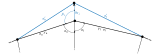
\includegraphics{img/model_development/node_shift_normal}
        \caption{Normal Direction}
        \label{fig:model_development/surface_normal}
    \end{subfigure}
    \begin{subfigure}{\linewidth}
        \centering
        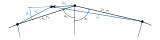
\includegraphics{img/model_development/node_shift_tangential}
        \caption{Tangential Direction}
        \label{fig:model_development/surface_tangential}
    \end{subfigure}
    \caption{Shifting of Surface Nodes}
    \label{fig:surface-node-shifting}
\end{figure}

\begin{figure}
    \begin{subfigure}{\linewidth}
        \centering
        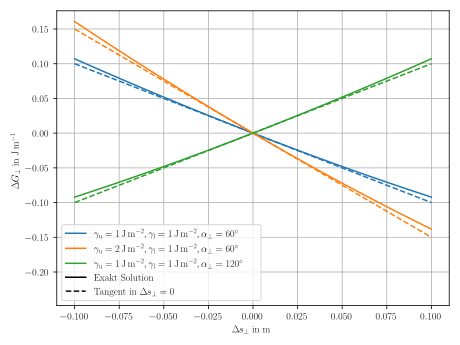
\includegraphics{img/model_development/plot_normal_potential}
        \caption{Normal Direction}
        \label{fig:model_development/plot_normal_potential}
    \end{subfigure}
    
    \begin{subfigure}{\linewidth}
        \centering
        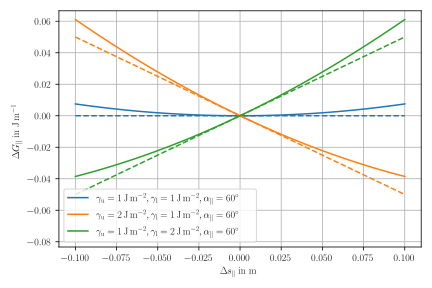
\includegraphics{img/model_development/plot_tangential_potential}
        \caption{Tangential Direction}
        \label{fig:model_development/plot_tangential_potential}
    \end{subfigure}
    \caption{Change in Gibbs Energy Due to Node Shifting (tangents dashed)}
    \label{fig:surface-node-potentials}
\end{figure}

If a node is displaced (shifted) in space, a change in Gibbs energy occurs due to the change in surface resp.\ interface area.
The amount of energy bound in a surface or interface is described by the interface energy $\InterfaceEnergy$.
Since a 2D problem is regarded, the length of the surface line $\SurfaceDistance$ is a measure of present surface area.
The change of Gibbs energy due to node shifting is described by \autoref{eq:gibbs-diff-surface-normal} with the prime values as measures after shifting.

\begin{equation}
  \Step\GibbsEnergy_\Normal = \left( \SurfaceDistance_{\Upper}' - \SurfaceDistance_{\Upper} + \SurfaceDistance_{\Lower}' - \SurfaceDistance_{\Lower} \right) \InterfaceEnergy_{\Surface}
    \label{eq:gibbs-diff-surface-normal}
\end{equation}

The shifting of nodes is separated into two components as shown in \autoref{fig:surface-node-shifting}.
The normal vector points under an angle of $\SurfaceVectorAngle_\Normal$ acc.~to~\autoref{eq:delta-surface-normal} to both surface lines.

\begin{equation}
  \SurfaceVectorAngle_{\Normal} = \pi - \frac{1}{2} \left(\SurfaceRadiusAngle_{\Upper} + \SurfaceRadiusAngle_{\Lower} \right)
    \label{eq:delta-surface-normal}
\end{equation}

With a certain normal shift ${\Step\Shift}_\Normal$, the surface lengths after shifting are calculated by \autoref{eq:surface-distance-shifted-normal-upper} and \autoref{eq:surface-distance-shifted-normal-lower}.

\begin{align}
  \SurfaceDistance_{\Upper}' &= \sqrt{\SurfaceDistance_{\Upper}^2 + \Step\Shift_{\Normal}^2 - 2 \SurfaceDistance_{\Upper} \Step\Shift_{\Normal} \cos \SurfaceVectorAngle_{\Normal}} \label{eq:surface-distance-shifted-normal-upper}\\
    \SurfaceDistance_{\Lower}' &= \sqrt{{\SurfaceDistance}_{\Lower}^2 + {\Step\Shift}_{\Normal}^2 - 2 {\SurfaceDistance}_{\Lower} {\Step\Shift}_{\Normal} \cos \SurfaceVectorAngle_{\Normal}} \label{eq:surface-distance-shifted-normal-lower}
\end{align}

The slope of the tangent in ${\Step\Shift}_{\Normal} = 0$ is calculated as in \autoref{eq:gibbs-partial-surface-normal}.
\autoref{fig:model_development/plot_normal_potential} shows the change in Gibbs energy due to normal shifting with different values of $\SurfaceVectorAngle_{\Normal}$ and $\InterfaceEnergy$.
A $\SurfaceVectorAngle_{\Normal} > \qty{90}{\degree}$ means a convex surface, thus energy gain when inward shifting (negative ${\Step\Shift}_{\Normal}$).
A $\SurfaceVectorAngle_{\Normal} < \qty{90}{\degree}$ means a concave surface, thus energy gain when outward shifting (positive ${\Step\Shift}_{\Normal}$).
A $\SurfaceVectorAngle_{\Normal} = \qty{90}{\degree}$ means a even surface, thus energy loss in both shifting directions.
Note, that the slope is dependent on the sum of ${\InterfaceEnergy}_{\Upper}$ and ${\InterfaceEnergy}_{\Lower}$, whereas the monotonicity depends on $\SurfaceVectorAngle_{\Normal}$.

\begin{equation}
    \frac{\partial \GibbsEnergy}{\partial {\Shift}_{\Normal}} = \lim_{\Step\Shift_{\Normal} \rightarrow 0} \frac{\Step\GibbsEnergy_{\Normal}}{\Step\Shift_{\Normal}} = -\left({\InterfaceEnergy}_{\Upper} + {\InterfaceEnergy}_{\Lower}\right) \cos \SurfaceVectorAngle_{\Normal}
    \label{eq:gibbs-partial-surface-normal}
\end{equation}

\begin{equation}
    \frac{\partial \Volume}{\partial {\Shift}_{\Normal}} = \frac{1}{2} \left( \SurfaceDistance_{\Upper} + \SurfaceDistance_{\Lower} \right) \sin \SurfaceVectorAngle_{\Normal}
    \label{eq:volume-partial-surface-normal}
\end{equation}

Regarding the normal shifting, the direction vector is under an angle of $\SurfaceVectorAngle_{\Tangential}$ acc.~to.~\autoref{eq:delta-surface-tangential} to the upper surface line.

\begin{equation}
    \SurfaceVectorAngle_{\Tangential} = \SurfaceVectorAngle_{\Normal} - \frac{\pi}{2}
    \label{eq:delta-surface-tangential}
\end{equation}

The change in Gibbs energy is calculated in a similar way acc.~to~\autoref{eq:gibbs-diff-surface-tangential}, but the shifted surface lengths calculate as in \autoref{eq:surface-distance-shifted-tangential-upper} and \autoref{eq:surface-distance-shifted-tangential-lower} in dependence on the tangential shift ${\Step\Shift}_{\Tangential}$.
Note the signs before the cosine terms.

\begin{equation}
    \Step\GibbsEnergy_{\Normal} = \left( \SurfaceDistance_{\Upper}' - \SurfaceDistance_{\Upper} + \SurfaceDistance_{\Lower}' - \SurfaceDistance_{\Lower} \right) \Surface{\InterfaceEnergy}
    \label{eq:gibbs-diff-surface-tangential}
\end{equation}

\begin{align}
    \SurfaceDistance_{\Upper}' &= \sqrt{{\SurfaceDistance}_{\Upper}^2 + {\Step\Shift}_{\Tangential}^2 - 2 {\SurfaceDistance}_{\Upper} {\Step\Shift}_{\Tangential} \cos \SurfaceVectorAngle_{\Tangential}} \label{eq:surface-distance-shifted-tangential-upper} \\
    \SurfaceDistance_{\Lower}' &= \sqrt{{\SurfaceDistance}_{\Lower}^2 + {\Step\Shift}_{\Tangential}^2 + 2 {\SurfaceDistance}_{\Lower} {\Step\Shift}_{\Tangential} \cos \SurfaceVectorAngle_{\Tangential}} \label{eq:surface-distance-shifted-tangential-lower}
\end{align}

The slope of the tangent in ${\Step\Shift}_{\Tangential} = 0$ is calculated as in \autoref{eq:gibbs-partial-surface-tangential}.
\autoref{fig:model_development/plot_tangential_potential} shows the change in Gibbs energy due to normal shifting with different values of $\InterfaceEnergy$.
The slope and monotonicity of these curves is here dependent on the \emph{difference} of ${\InterfaceEnergy}_{\Upper}$ and ${\InterfaceEnergy}_{\Lower}$.
The convexity or concavity of the surface is here only of minor importance.
Whether the interface with higher $\InterfaceEnergy$ is located on the upper or lower side determines the monotonicity of the curves.
In the special case when ${\InterfaceEnergy}_{\Upper} = {\InterfaceEnergy}_{\Lower}$, the curve has a minimum in ${\Step\Shift}_{\Tangential} = 0$, meaning that any shift will produce an energy loss.
This is the case on all nodes except neck nodes.

\begin{equation}
    \frac{\partial \GibbsEnergy}{\partial {\Shift}_{\Tangential}} = \lim_{\Step\Shift_{\Tangential} \rightarrow 0} \frac{\Step\GibbsEnergy_{\Tangential}}{\Step\Shift_{\Tangential}} = -\left({\InterfaceEnergy}_{\Upper} - {\InterfaceEnergy}_{\Lower}\right) \cos \SurfaceVectorAngle_{\Tangential}
    \label{eq:gibbs-partial-surface-tangential}
\end{equation}

\begin{equation}
    \frac{\partial \Volume}{\partial {\Shift}_{\Tangential}} = \frac{1}{2} \left( \SurfaceDistance_{\Lower} - \SurfaceDistance_{\Upper} \right) \sin \SurfaceVectorAngle_{\Tangential}
    \label{eq:volume-partial-surface-tangential}
\end{equation}
